\documentclass[11pt, twoside]{report}
\usepackage[utf8]{inputenc}
\usepackage[margin=2.5cm]{geometry}
\usepackage{graphicx}  		% display images
\usepackage{rotating}
\usepackage{natbib}
\usepackage{tikz} 
\usepackage[portuguese]{babel}
\usepackage{indentfirst}
\usepackage[colorlinks=true,linkcolor=black,urlcolor=black,bookmarksopen=true]{hyperref} % Make hyperlinks in index
\usepackage{bookmark} 		% Bookmarks for pdf file
\usepackage{float} 			% colocar as imegens e tabelas dentro do texto
\usepackage{fancyhdr}
\pagestyle{fancy}
\usepackage{tabularx} 		% x column in table can jump a line
\usepackage{setspace} 		% espçamento entre linhas
\usepackage{fancyhdr} 		% creates fancy footers and headers
\raggedbottom				% makes bottom of page more empy to make sure previous text doesnt have vertical gaps
\usepackage{ltablex}
\usepackage{pdflscape}
\pagestyle{fancy}
\lfoot{{\footnotesize Tecnologias de Informação}}
\rfoot{{\footnotesize ESTGA}}
\rhead{PTDW}
\lfoot{Calendário de exames}

\renewcommand{\footrulewidth}{1pt}%criar uma linha no que separa o rodapé
%\usepackage{appendix}
%\noindent %sem indentação
%\newcommand{\annexname}{Anexo}
%\makeatletter % treat @ as a letter instead of a control word.
%
%\newcommand\annex{\par
%	\setcounter{chapter}{0}
%	\setcounter{section}{0}
%	\renewcommand\appendixname{Anexo}
%	\renewcommand\appendixpagename{Anexos}
%	\renewcommand{\appendixtocname}{Anexos}
%	\gdef\@chapapp{\annexname}
%	\gdef\thechapter{\@Roman\c@chapter}
%	\renewcommand{\theHchapter}{\annexname.\thechapter}
%	\addappheadtotoc
%}\makeatother


\usepackage{multirow}
\begin{document}
	
\onehalfspacing % espaçamento de 1,5 entre linhas

	
%	\lhead{Escola Superior de Tecnologia e Gestão de Águeda\\
%		Licenciatura em Tecnologias da Informação
%	}
	
	%\rhead{Capítulo \thechapter}
	\pagenumbering{roman}
	
	\begin{titlepage}
		\centering
		\scshape\Huge Calendário Exames\par
		\vspace{0.9cm}
		
		\scshape\large Projeto Temático em Desenvolvimento Web \\
		\vspace{0.3cm}
		\scshape\large 1º semestre de 2021/2022\par
		\vspace{0.4cm}
		\centering
		%\includegraphics[width=10cm]{}\par
		
		\vspace{1cm}
		
		\large
		Autores\\
		Gonçalo Tavares, Nº 92382  \\
		Bruno Lopes, Nº 86217 \\
		Leonardo Silva, Nº 95381 \\
		Ricardo Fernandes, Nº 49880 \\
		Sofia Rocha, Nº 99991 \\
		
		\vspace{1cm}
		
		\centering
		
\includegraphics[width=10cm]{image/AssB_vertical_cor.png}
		
		\newpage
		\thispagestyle{plain}%retira cabeçalho e rodape
		\thispagestyle{empty}%retira a numeração da pagina
		\centering
		\scshape\Huge Calendário Exames \par
		\vspace{1cm}
		
		\scshape\large Projeto Temático em Desenvolvimento Web\par
		\vspace{1cm}
		\scshape\large 1º semestre de 2021/2022\par
		\vspace{4cm}
		
		
		
		\large
		Autores\\
		Bruno Lopes, Nº 86217 \\
		Gonçalo Tavares, Nº 92382  \\
		Leonardo Silva, Nº 95381 \\
		Ricardo Fernandes, Nº 49880  \\
		Sofia Rocha, Nº 99991 \\
		
		\vspace{1cm}
		Orientadores\\
		Rita Santos \\
		Fábio Marques\\
		\vspace{4cm}
		
		\centering
		
\includegraphics[width=10cm]{image/AssB_vertical_cor}
		
	\end{titlepage}

	\newpage
	\setcounter{page}{1} % começa a contar a paginas no numero 1
	\tableofcontents % Índice de conteúdos
	\thispagestyle{plain} % retira cabeçalho e rodape
	\thispagestyle{empty} % retira a numeração da pagina
	\newpage
	\listoftables % Lista de tabelas
	\newpage
	\listoffigures % Lista de figuras
	
	\newpage
	\pagenumbering{arabic}
	
	\chapter{Introdução}
	
	No âmbito do Projeto Temático em Desenvolvimento Web com as disciplinas Web Design e Desenvolvimento Web Multiplataforma foi-nos proposto o desenvolvimento de uma das seguintes aplicações: gestão de cacifos ou criação dos calendários de avaliações. Por votação a maioria escolheu a criação de calendários de avaliações.
	
	Este projeto consiste em criar calendários de exames a partir de uma plataforma web.
	\section{Objetivos da aplicação}
	metodologia de trabalho
	
	Criação de calendários de exames
	
	\chapter{Estado de arte}
	
	
	dizer que foi dificil encontrar
	
	\chapter{Planificação do projeto}

 	

	\chapter{Análises dos utilizadores e tarefas}
	
	Após a primeira renuião com o cliente chegou-se à conclusão que  este é também um potencial utilizador e que tem uma ideia precisa das funcionalidades da aplicação. Por isso, aliado à restrição de tempo achou-se que não se iria aprofundar na análise dos utilizadores. 
	
	O cliente no momento recorre ao excel para a criação de calendários,  colocando todas as salas, cursos e etc com alto risco de erro e com baixa eficiência. Para além disso a formatação final (em .pdf) também é feita pelo excel.

	
	



	processo atual da criação dos calendários de exames
	reunião com o cliente
	
	\chapter{Modelo de requisitos}
	\section{Requisitos funcionais}
	
	
	Os requisitos funcionais representam todas as funcionalidades que o sistema pode fazer ou que o utilizador pode realizar no sistema. Com isso na tabela \ref{requisitiosfuncionais} estam todos os requisitos funcionais dividos por várias categorias: importação, exportação, marcação de exames, configurações, avisos, pesquisa e outros (requisitos que não se encaixam em nenhuma das categorias descritas). Dentro da categoria "avisos" tem as funcionalidades que o sistema irá realizar após uma ação do utilizador, ao contrário de todas as outras categorias em que o utilizador tem a possibilidade realizar determinada tarefa.
	
	Para além disso os requisitos funcionais estam classificados por prioridade sendo os de alta prioridade realizados nas primeiras fases e os de baixa prioridade implementados nas últimas fases (ver secção \ref{selecaocasosdeuso}).  
	
	
	
\def\arraystretch{1.5}%
	\begin{center}
		\label{requisitiosfuncionais}
		\begin{longtable}{|m{1cm}|m{2.2cm}|m{10cm}|m{2cm}|}
			\caption{Requisitos funcionais}\\
			
			\hline			
			\textbf{Refª }	& \textbf{Categoria}&\textbf{Descrição do requisito} & \textbf{Prioridade} \\
			\hline
			
			
			RF.1 &Importação& Importação de ficheiros com a configuração de salas, disciplinas e docentes em formato .csv & Alta \\
			\hline
			
			RF.2 &\multirow{2}{2cm}{Exportação}& Exportação de calendários em formato .pdf & Alta \\
			
			RF.3 && Exportação o calendário em língua Inglesa & Baixa \\
			\hline
			
			RF.4 &\multirow{7}{2cm}{Marcação de exames}& Os exames podem ser marcados em três turnos: manhã (às 9h30), tarde (às 14h) e noite (às 18h30) por padrão & Alta \\
			
			RF.5 && O utilizador pode associar vigilantes a cada exame & Alta \\
			
			RF.6 && Criação épocas de avaliação adicionando um nome e uma data de início e fim & Alta \\
			
			RF.7 && O calendário não deverá permitir a marcação de exames aos domingos e feriados & Alta \\
			RF.8 &&O utilizador pode associar a cada exame vários vigilantes & Alta\\
			
			RF.9 &&	O utilizador pode associar mais do que uma sala a um exame & Alta\\
			
			RF.10 && Se houver vários cursos com o mesmo exame então será associado a todos os calendários dos cursos associados. & Média\\
			\hline
		
			RF.11. &\multirow{6}{2cm}{Configurações}& Configurar tipo de sala com equipamento e lotação total & Alta \\
			
			RF.12. & 	& Inserção de cursos e disciplinas & Alta\\
			
			RF.13. && Permitir inserir novos docentes & Alta\\
			
			RF.14. && Permitir editar informações (nome, que disciplinas está a lecionar, horário de trabalho) sobre os docentes & Alta\\
			
			RF.15. && Permitir colocar restrições arbitrárias introduzidas pelo utilizador & Baixa \\
			
			RF.16. && Permitir associar na área do docente dias em que os mesmos não estão disponíveis & Alta\\
			
			\hline
			
			RF.17 &\multirow{9}{2cm}{Avisos}& Aparecimento de um aviso no caso de incongruência da informação durante a marcação de exames & Alta \\
			
			RF.18 &&Mostrar um aviso de alta prioridade se houver sobreposições de exames & Alta\\
			
			RF.19 && Mostrar um aviso de alta prioridade se o docente não estiver disponível & Alta \\
			
			RF.20 && Mostrar um aviso de alta prioridade se a sala não estiver disponível & Alta\\
			
			RF.21 && Mostrar um aviso de alta prioridade se o curso for diurno e colocar um exame no turno da noite e vice-versa & Média\\
			
			RF.22&&Mostrar um aviso de alta prioridade se o docente associado ao mesmo exame for repetido & Alta \\
			
			RF.23 && Mostrar um aviso de alta prioridade se o exame necessitar de uma sala de informática e não for associada sala desse tipo & Média\\
			
			RF.24 && Mostrar um aviso de alta prioridade se houver mais alunos inscritos do que  lotação máxima da sala & Alta\\
			
			RF.25 && Mostrar um aviso de média prioridade se houver exames marcados no mesmo dia e hora do mesmo curso mas anos diferentes & Média\\
			\hline
			
			RF.26 &Autenticação& O utilizador só pode aceder à aplicação após a autenticação & Alta\\
			\hline
			RF.27 &\multirow{2}{*}{Pesquisa}& O utilizador pode utilizar um ou mais filtros na pesquisa de calendários & Alta\\
		
			RF.28  && Pesquisar por calendários com filtro por cursos, ano, semestre e época de avaliação  & Alta \\
			\hline
			
			RF.29 &\multirow{2}{*}{Outros}& A criação de um novo calendário deverá sempre partir do início sem nenhuma configuração associada & Alta\\
		
			RF.30 && Guardar e visualizar calendários de exames de anos anteriores sem informações específicas (perguntar ao Paulo) & Média \\
			\hline
		\end{longtable}
	\end{center}



	
	\section{Requisitos não funcionais}
	
	Os requisitos não funcionais estam dividos em três categorias: requsitos de interface e facilidade de uso que representam todos os requisitos que melhorem a usabilidade da aplicação; requisitos de segurança e integridade dos dados e requisitos de interface com sistemas externos e ambientes de execução.
	
	\subsection{Requisitos de interface e facilidade de uso}

	
	\begin{table}[H]
	\caption{Requisitos de interface e facilidade de uso}
	
	\begin{center}
		\begin{tabularx}{\textwidth}{|c|X|c|}
			\hline
			\textbf{Refª }	& \textbf{Descrição do requisito} & \textbf{Prioridade} \\
			\hline
			RIF1 & As disciplinas e cursos podem ser inseridas através de \textit{drag e drop} &Alta\\
			\hline
			RIF2 & Interface responsiva permitindo a sua visualização em ambiente mobile &Alta\\
			\hline
			RIF3 & Linguagem padrão em Português de Portugal &Alta\\
			\hline
			RIF4 & Há dois tipos de avisos distinguidos com texto e cor &Alta\\
			\hline
		\end{tabularx}
		\label{requisitosdeinterface}
	\end{center}
	\end{table}

	\subsection{Requisitos de segurança e integridade dos dados}
	
	perfil secretaria 
perfil admin

possibilidade de criar novos utilizadores
rede da ua

perguntar ao cliente
\begin{table}[H]	
	\caption{Requisitos de segurança e integridade dos dados}
	
	
	\begin{center}
		\begin{tabularx}{\textwidth}{|c|X|c|}
			\hline
			\textbf{Refª }	& \textbf{Descrição do requisito} & \textbf{Prioridade} \\
			\hline
			RSI1 &O histórico não pode ter associações a outras tabelas da base de dados  &Alta\\
			\hline
			RSI2 & Uma única conta de utilizador&\\
			\hline
		\end{tabularx}
		\label{requisitosdeseguranca}
	\end{center}
\end{table}


	\subsection{Requisitos de interface com sistemas externos e ambientes de execução}
	
	
	
	
	\begin{table}[H]
		\caption{Requisitos de interface com sistemas externos e ambientes de execução}
		\begin{center}
			\begin{tabularx}{\textwidth}{|c|X|c|}
				\hline
				\textbf{Refª }	& \textbf{Descrição do requisito} & \textbf{Prioridade}\\
				\hline
				RSA1 & Suportar Browsers com motor renderização webkit/blink (Chrome, Edge, Safari, Brave, etc.)  & Alta \\
				\hline
				RSA2 & Suportar Firefox ESR e outros derivados de gecko/quantum & Alta \\
				\hline
				RSA5 & Ter acesso à Internet (precisa mesmo? rede interna UA não é suficiente?) & Alta\\
				\hline
			\end{tabularx}
			\label{requisitosdesistemas}
		\end{center}
	\end{table}
		
	
	\chapter{Modelo de casos de utilização}
	\section{Diagrama de casos de utilização}
	
\clearpage
\begin{landscape}
	\pagestyle{empty}
	
		\begin{figure}[H] 
			\centering 			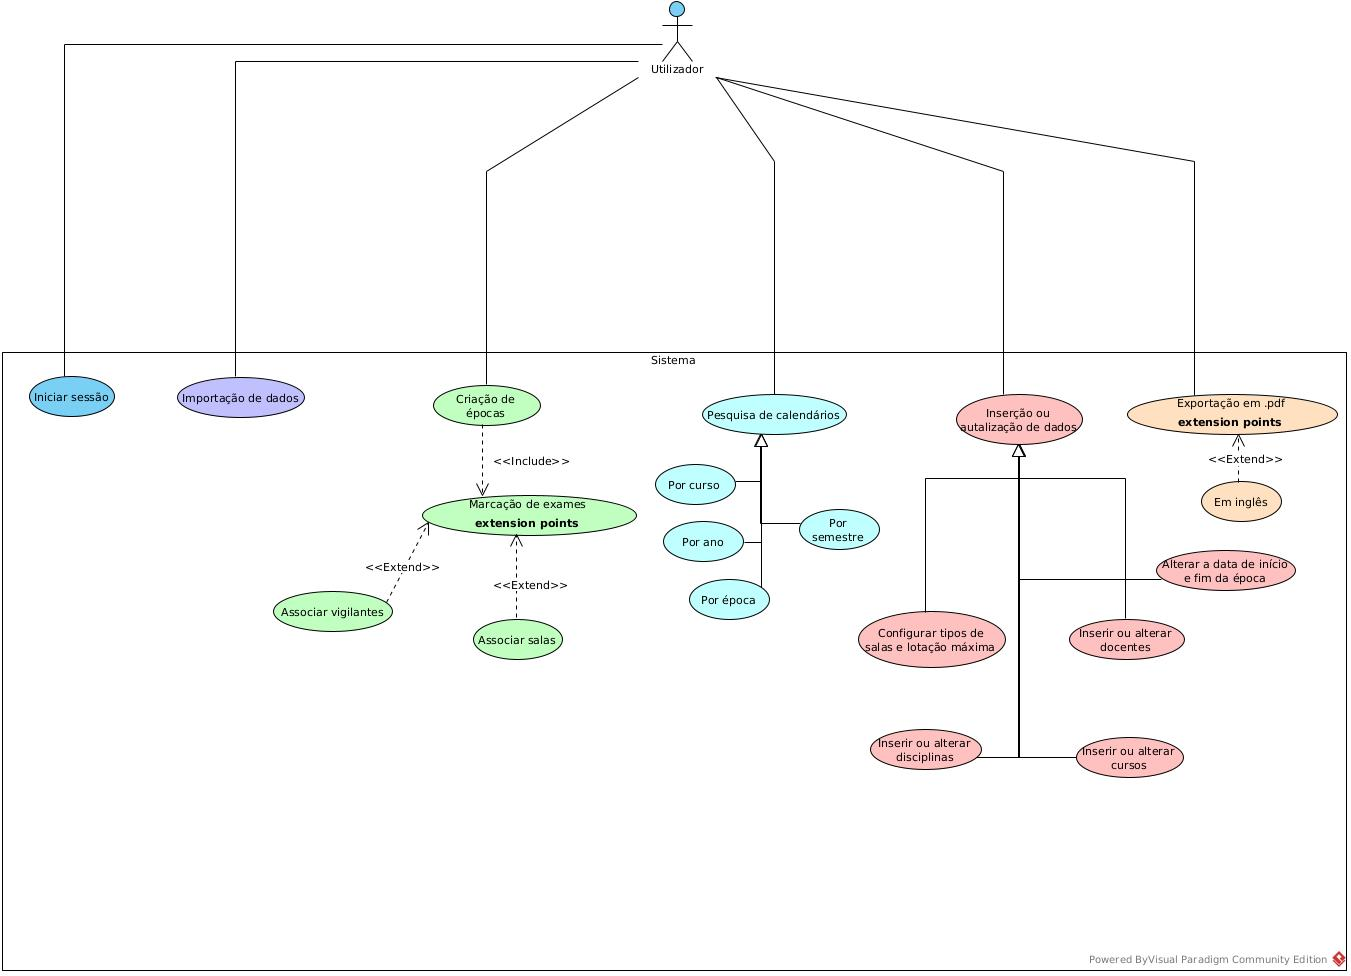
\includegraphics[width=1.3\textwidth,height=1.3\textheight,keepaspectratio]{image/diagrama}
			\caption{Diagrama dos casos de utilização}
		
		\end{figure}
\end{landscape}


	\section{Seleção dos casos de utilização}
	\label{selecaocasosdeuso}
	Os casos de utilização da primeira fase:
	
	\begin{itemize}
		\item Autenticação;
		\item Importação de ficheiros .csv com a configuração de salas, disciplinas e docentes;
	 	\item Criação de épocas com data de início e fim;
	 	\item Configuração dos tipos de salas e a lotação máxima;
	 	\item Marcação de exames através de \textit{drag \& drop}  no calendário.
	 	\item Pesquisa de calendários por curso, ano, semestre e época de avaliação;
	\end{itemize}
	
	Segunda fase:
	\begin{itemize}
		\item Inserção de cursos e disciplinas;
		\item Restringir a marcação de exames ao domingos e feriados;
		\item Associar um ou mais docentes aos exames para serem vigilantes;
		\item Inserção de novos docentes;
		\item Associar uma ou mais salas a um exame;
		\item Exportação do calendário em formato pdf;
	\end{itemize}


	Terceira fase:
	\begin{itemize}
		\item Associar na área de docentes dias em que os mesmos não estão disponíveis;
		\item Editar informações sobre os docentes;
		\item Avisar se houver sobreposição de exames;
		\item Avisar se o docente não estiver disponível;
		\item Avisar se houver mais alunos inscritos do que a lotação máxima da sala;
		\item Avisar se a sala não estiver disponível;
		\item Avisar caso o docente associado ao exame for repetido;
	\end{itemize}
	
	Quarta fase:
	\begin{itemize}
		\item Avisar se o curso for diurno e houver uma marcação para o turno da noite e vice-versa.
		\item Associar o mesmo exame a todos os cursos que têm a mesma disiplina.
		\item Avisar caso o tipo de sala associada ao exame não for apropriada (informática ou normal)
		\item Exportação do calendário em inglês
	\end{itemize}

	
	\section{Descrição dos casos de utilização}
	
	
		
	\begin{table}[H]
		\caption{Caso de utilização - autenticação}
		\begin{center}	
			\begin{tabularx}{\textwidth}{|l|X|}
				\hline
				\textbf{Nome }	& \textbf{Autenticação} \\
				\hline
				Atores: & Utilizador \\
				\hline
				Prioridade: & Alta \\
				\hline
				Requisitos funcionais:&  \\
				\hline
				Finalidade: & Aceder às funcionalidades da aplicação\\
				\hline
				Sumário: &  \\
				\hline
				Pré-condições: & Ter uma conta registada na aplicação e estar dentro da rede da UA\\
				\hline
				Descrição da interação: &  O utilizador assim que abre a aplicação tem de iniciar a sessão com o seu email e palavra-passe correspondentes\\
				\hline
				Cenário alternativo:&\\
				\hline
			\end{tabularx}
		\end{center}
	\end{table}

	
\begin{table}[H]
	\caption{Caso de utilização - importação de ficheiros}
	\begin{center}	
		\begin{tabularx}{\textwidth}{|X|X|}
			\hline
			\textbf{Nome }	& \textbf{Importação de ficheiros}\\
			\hline
			Atores: & Utilizador\\
			\hline
			Prioridade: &  Alta\\
			\hline
			Requisitos funcionais:&  \\
			\hline
			Finalidade: &  Importação de dados para atualizar a base de dados.\\
			\hline
			Sumário: &O utilizador pode importar dados sobre os docentes, disciplinas e cursos, atualizando a base de dados, através de um ficheiros .csv. \\
			\hline
			Pré-condições: & Ter iniciado sessão na aplicação e ter o ficheiro .csv com os dados correspondentes\\
			\hline
			Descrição da interação: &  \\
			\hline
			Cenário alternativo 1 - não é possível ler o ficheiro &Irá mostrar uma mensagem de erro.\\
			\hline
			Cenário alternativo 2 - o ficheiro adicionado não é do formato .csv &Irá mostrar uma mensagem de erro que não é possível importar ficheiros que não sejam do tipo .csv\\
			\hline
		\end{tabularx}
	\end{center}
\end{table}




\begin{table}[H]
	\caption{Caso de utilização - criação de épocas de avaliação}
	\begin{center}	
		\begin{tabularx}{\textwidth}{|l|X|}
			\hline
			\textbf{Nome }	& \textbf{Criação de épocas de avaliação} \\
			\hline
			Atores: & Utilizador\\
			\hline
			Prioridade: &  Alta\\
			\hline
			Requisitos funcionais:&  \\
			\hline
			Finalidade: & Criação de épocas (com data de início e fim) para a realização de exames. \\
			\hline
			Sumário: & O utilizador pode criar épocas de exames para os vários cursos. Cada época estará associada a um ano, semestre e um nome dado pelo utilizador.\\
			\hline
			Pré-condições: & Ter iniciado sessão na aplicação.\\
			\hline
			Descrição da interação: &  \\
			\hline
			Cenário alternativo: &\\
			\hline
		\end{tabularx}
	\end{center}
\end{table}


\begin{table}[H]
	\caption{Caso de utilização - marcação de exames}
	\begin{center}	
		\begin{tabularx}{\textwidth}{|l|X|}
			\hline
			\textbf{Nome }	& \textbf{Marcação de exames} \\
			\hline
			Atores: & Utilizador\\
			\hline
			Prioridade: &  Alta\\
			\hline
			Requisitos funcionais:&  \\
			\hline
			Finalidade: & Marcação de exames na época de avaliações\\
			\hline
			Sumário: & O utilizador pode marcar os exames na época de avaliações escolhida. Pode marcar num dos três turnos: manhã, tarde e noite.\\
			\hline
			Pré-condições: & Ter iniciado sessão na aplicação, ter importado ou adicionado informações sobre os cursos, disciplinas, docentes e salas e ter escolhido o curso e a época de avaliações.\\
			\hline
			Descrição da interação: &  \\
			\hline
			Cenário alternativo: &\\
			\hline
		\end{tabularx}
	\end{center}
\end{table}


	
	

\begin{table}[H]
	\caption{Caso de utilização - pesquisa de calendários}
	\begin{center}	
		\begin{tabularx}{\textwidth}{|l|X|}
			\hline
			\textbf{Nome }	& \textbf{Pesquisa de calendários} \\
			\hline
			Atores: & Utilizador\\
			\hline
			Prioridade: &  Alta\\
			\hline
			Requisitos funcionais:&  \\
			\hline
			Finalidade: & Pesquisa de calendários através de filtros.\\
			\hline
			Sumário: & O utilizador pode pesquisar entre todos os calendários criados através de filtros como o curso, ano, semestre ou ano.\\
			\hline
			Pré-condições: & Ter iniciado sessão na aplicação e ter criado calendários de avaliação\\
			\hline
			Descrição da interação: &  \\
			\hline
			Cenário alternativo: &\\
			\hline
		\end{tabularx}
	\end{center}
\end{table}


	
	\chapter{Prototipagem}
	\section{Protótipo de baixa fidelidade}
	\subsection{Wireframes}
	\subsection{Diagrama de user flow}
	\subsection{Testes}
	\subsubsection{Análise de resultados}
	
	\section{Protótipo de alta fidelidade}
	\subsection{Desenvolvimento do protótipo}
	\subsection{Guia de estilos}
	\subsection{Testes}
	\subsubsection{Análise de resultados}
	
	\chapter{Implementação do modelo de dados persistentes}
	\section{Estrutura da base de dados}
	\subsection{Base de dados - factories}
	\section{Arquitetura do sistema - Modelo MVC}
	\subsection{Models e Controllers}
	
	\chapter{Primeira versão da aplicação}
	\section{Implementação de funcionalidades}
	
	\chapter{Testes finais}
	\section{Testes com potenciais clientes}
	\section{Testes de acessibilidade}
	\section{Análise de resultados}
	
	\chapter{Lançamento da versão final}
	\section{Alocação da aplicação no servidor}
	
	\pagebreak
	wasd
	wasd
	
	
	wasd
	
	
	\pagebreak
	
	asd
	
	wasd
	\chapter{Reflexão crítica e conclusão}
	
	

	\bibliographystyle{ieeetr}
	\bibliography{}
	
\end{document}	
	
	
	
	
